% !TeX encoding = UTF-8
\chapter[Nützliche Latex-Informationen]{Nützliche Latex-Informationen (Verwendung ist optional)}

\section{Latex-Distributionen und Editoren}

\LaTeX-Pakete und -Kompilierer haben den Vorteil, dass sie vollständig unabhängig von dem später verwendeten Latex-Editor installiert werden können. Sie werden in sogenannten Latex-Distributionen zusammengefasst. Empfehlenswerte Distributionen sind unter Windows MikTeX (\href{http://miktex.org/}{http://miktex.org/}) und unter OS~X MacTeX \href{https://tug.org/mactex/}{https://tug.org/mactex/}.

Die Auswahl des Latex-Editors erfolgt in der Regel nach individuellen Bedürfnissen und Geschmack.
Ein empfehlenswerter, plattformübergreifender Editor ist TeXstudio \href{http://texstudio.sourceforge.net/}{http://texstudio.sourceforge.net/}. Dieser bietet unter anderem die Möglichkeit, gewünschte Positionen der PDF-Vorschau unmittelbar im Quelltext anzuzeigen.
Ein weiterer verbreiteter Editor ist TeXnicCenter (\href{http://www.texniccenter.org/}{http://www.texniccenter.org/}).

Abschließend muss sich der Autor zwischen dem Latex- (PS/Dvi) und dem Pdflatex-Kompilierer entscheiden.
Die jeweilige Auswahl ist in den Einstellungen des verwendeten Editors zu treffen.\\

Pdflatex:
\begin{itemize}
	\item Fortschrittlicher als Latex
	\item Unterstützt folgende Bilddateitypen: PDF (Vektor), PNG, JPG.
	\item Unterstützt EPS-Bilder mit dem Paket "`epstopdf"' (bereits inkludiert).
	\item Nicht kompatibel mit alten Paketen, die nur mit PostScript-Dateien arbeiten.
\end{itemize}

Latex (PS/Dvi):
\begin{itemize}
	\item Funktioniert mit "`psfrag"' und anderen auf PS basierenden Paketen.
	\item Unterstützt ohne weitere Konvertierungen nur EPS-Bilder.
	\item Längere Kompilierungszeit
\end{itemize}


\section{Bild neben Tabelle}
Eine Tabelle neben einer Abbildung einfügen unter Berücksichtigung der zugehörigen Verzeichnisse (Tabellen, Abbildungen):
\begin{figure}[htbp]
%
	\begin{minipage}[t]{0.45\textwidth}
	\centering
	\raisebox{2.5cm}{ %per hand
		\begin{tabular}{cc}
		\toprule
		Konfiguration & Parametersatz \\
		\midrule
		$1$ & $\{p_{1}, \: p_{2}, \: p_{5}\}$ \\
		$2$ & $\{p_{1}, \: p_{4}, \: p_{5}\}$ \\
		$3$ & $\{p_{2}, \: p_{3}, \: p_{4}\}$ \\
		\bottomrule
		\end{tabular}
	}
	\captionof{table}{Definitionsbereich der Parameter zur Optimierung.} %ins tabellenverzeichnis einfügen
	\label{tab:bsp2}
	\end{minipage}
%
	\begin{minipage}[t]{0.45\textwidth}
	\centering
	  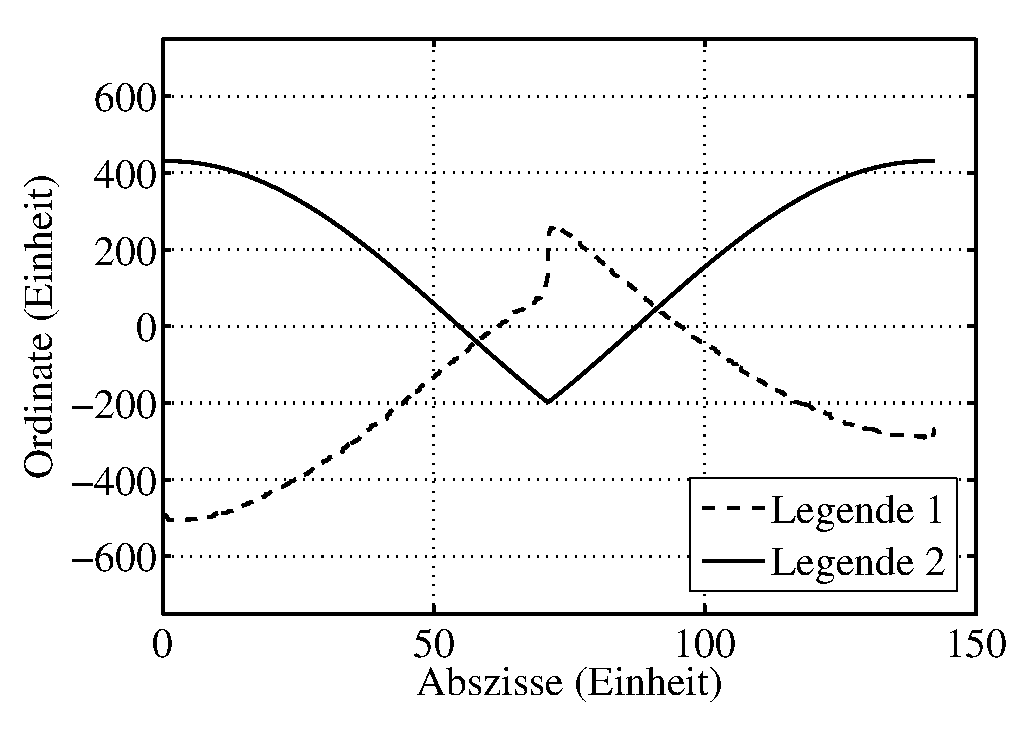
\includegraphics[width=\textwidth]{pic1}
  	\captionof{figure}{Musterdiagramm}
	\end{minipage}
\end{figure}


\section{Subcaption: Bild neben Bild und Tabelle neben Tabelle}

Das \textit{Subcaption} package (Beschriftung von Tabellen und Abbildungen mit a), b), ...) sollte ausschließlich gewählt werden,
wenn die zugehörigen Tabellen / Abbildungen auch wirklich kontextuell zusammengehören.

\begin{figure}[htbp]
        \centering
        \begin{subfigure}[b]{0.3\textwidth}
        		\centering
                
\includegraphics[width=\textwidth]{logos/tud_logo_rgb} 
                \caption{TU Dortmund Logo}
                \label{fig:subfigure_tud_logo}
        \end{subfigure}%
        \quad %add desired spacing between images, e. g. ~, \quad, \qquad, \hfill etc.
          %(or a blank line to force the subfigure onto a new line)
        \begin{subfigure}[b]{0.3\textwidth}
        		\centering
                
\includegraphics[width=0.3\textwidth]{logos/rst_rgb} % relative width w.r.t. to the subfigure box
                \caption{RST Logo}
                \label{fig:subfigure_rst_rgb}
        \end{subfigure}
        \caption{Sammlung aller Logos}
        \label{fig:logos}
\end{figure}

Für lange Beschreibungstexte kann die \textit{Subfigure-Caption} leer gelassen werden. Eine Beschreibung mit Referenz zu den Buchstaben a),..., erfolgt dann in der allgemeinen Beschreibung.

Tabelle \ref{tab:parameter_tabellen} listet alle verwendeten Parameter auf. Tabelle \ref{tab:parameter_tabelle1} ...

\begin{table}[htbp]
\caption{Hauptbeschriftung}
\centering
	\begin{subtable}[t]{.5\textwidth}
	\centering
			\caption{Tabelle links}
			\begin{tabular}{cc}
				\toprule
				Konfiguration & Parametersatz \\
				\midrule
				$1$ & $\{p_{1}, \: p_{2}, \: p_{5}\}$ \\
				$2$ & $\{p_{1}, \: p_{4}, \: p_{5}\}$ \\
				$3$ & $\{p_{2}, \: p_{3}, \: p_{4}\}$ \\
				\bottomrule
			\end{tabular}
			\label{tab:parameter_tabelle1}
	\end{subtable}%
	\begin{subtable}[t]{.5\textwidth}
			\centering
			\caption{Tabelle rechts}
			\begin{tabular}{cc}
				\toprule
				Konfiguration & Parametersatz \\
				\midrule
				$1$ & $\{p_{1}, \: p_{2}, \: p_{5}\}$ \\
				$2$ & $\{p_{1}, \: p_{4}, \: p_{5}\}$ \\
				$3$ & $\{p_{2}, \: p_{3}, \: p_{4}\}$ \\
				\bottomrule
			\end{tabular}
			\label{tab:parameter_tabelle2}
	\end{subtable}
	\label{tab:parameter_tabellen}
\end{table}




%
%
%
%%%%%%%%%%%%%%%%%%%%%%%%%%%%%%%%%%%%%%%%%%%%
\clearpage
\section{Zeichnungen und Matlab-Plots mit Tikz}
\label{sec:tikz}

Tikz ist ein umfangreiches \LaTeX-Paket, mit dem Bilder über Programmanweisungen erstellt werden können.
Zahlreiche Anleitungen und Beispiele können unter dem folgenden Link eingesehen werden:\\ 
\href{http://www.texample.net/tikz/examples/}{\emph{http://www.texample.net/tikz/examples/}}
\\

Eine besonders nützliche Anwendung entsteht aus der Kombination mit dem Matlab-Plugin "`matlab2tikz"':\\
\href{http://www.mathworks.com/matlabcentral/fileexchange/22022-matlab2tikz}{\emph{http://www.mathworks.com/matlabcentral/fileexchange/22022-matlab2tikz}}\\
Hiermit können in Matlab erstellte Bilder in ein Tikz-Bild umgewandelt werden. Ein Vorteil ist die einfache Möglichkeit, anschließend beliebige Attribute des Bildes beziehungsweise der Zeichnung anzupassen: Linienfarbe, -breite, -typ, Gitter, Legenden, Marker, u.a.

Die prinzipielle Vorgehensweise ist wie folgt:
\begin{enumerate}
	\item Matlab Zeichnung erstellen und in den Vordergrund holen (am Besten alle anderen Bilder schließen).
		Attribute der Zeichnung können auch schon hier angepasst werden (Gitter, Linienfarbe, -breite, Log-Skalierung,...).
	\item Nachdem "`matlab2tikz"' in den Matlab-Pfaden hinzugefügt wurde, kann das Bild konvertiert werden:\\
		\textit{matlab2tikz('myfile.tikz', 'height', '\textbackslash figureheight', 'width', '\textbackslash figurewidth');} \\
		Die Variablen \textbackslash figureheight und \textbackslash figurewidth erlauben die spätere beliebige Anpassung der Größe des Bildes.
	\item \textit{myfile.tikz} in das Abbildungsverzeichnis dieser Arbeit kopieren.
	\item Tikz-Bild nach dem unten aufgeführten Beispiel einbinden (siehe Quellcode).
	\item \textit{myfile.tikz} beliebig verändern. Google hilft bei vielen speziellen Wünschen. 
\end{enumerate}


\begin{figure}[h]
\centering
%\tikzexternaldisable
\includetikz[0.9\textwidth][5cm]{x_square} %[width][height][filename without ./Abbildungen/...)]
\caption{Quadratische Funktion}
\label{fig:tikz:x_square}
\end{figure}


\subsection{Tikz-Plots anpassen}

Falls \texttt{matlab2tikz} verwendet wird, verwendet die Tikz-Umgebung zunächst die wissenschaftliche Darstellung von Zahlen, d.h. abhängig von Zehnerpotenzen.
Ist dies nicht gewünscht, können in die \textit{axis}-Umgebung die folgenden Befehle, oder eine Auswahl davon, eingefügt werden:

\begin{itemize}
         \item \texttt{scaled y ticks = false,} 
         \item \texttt{scaled x ticks = false,}
         \item \texttt{y tick label style={/pgf/number format/.cd, fixed, int detect, fixed zerofill, precision=3},}
         \item \texttt{x tick label style={/pgf/number format/.cd, fixed, int detect, fixed zerofill, precision=3}}
\end{itemize}

Die ersten zwei Befehle erlauben die Zusammenfassung der Zehnerpotenzen, sodass eine gemeinsame Zehnerpotenz an die Achse geschrieben wird.
Die unteren beiden Befehle stellen die notwendige Präzision ein.

\subsection{Tikz externalisieren}

Wer viele Tikz-Bilder einbindet oder Tikz-Bilder mit einer sehr großen Anzahl an Datenpunkten verwendet, der wird zwangsläufig 
auf lange Kompilierungszeiten beziehungsweise Abbrüche aufgrund eines überfüllten Latex-Zwischenspeichers stoßen.

Um dieses Problem zu vermeiden und die Kompilierungszeit erheblich zu erhöhen, bietet Tikz die Möglichkeit, Bilder vorzukompilieren. Damit werden vollautomatisiert eps/pdf Bilder aus dem Tikz-Quelltext erzeugt und anschließend intern eingebunden.
Die notwendigen Konfigurationen sind in "`packages.tex"' bereits voreingestellt. Die einzige, benutzerseitige Änderung erfolgt im verwendeten Latexeditor. Dem Latex- beziehungsweise PdfLatex-Kompilierer muss die Erlaubnis erteilt werden,
Shell-Scripte auszuführen.
Dazu die Argumentliste in den Editor-Einstellungen um folgenden kompilierer- und systemspezifischen Eintrag erweitern:\\

Bei Windows-Systemen (MikTeX):
\begin{itemize}
	\item	\textit{latex.exe [other arguments] -enable-write18 \%.tex}
 	\item 	\textit{ pdflatex.exe [other arguments] -enable-write18 \%.tex}
\end{itemize}

Bei Unix-Systemen (MacTeX/Linux):
\begin{itemize}
	\item	\textit{latex.exe [other arguments] -shell-escape \%.tex}
	\item 	\textit{pdflatex.exe [other arguments] -shell-escape \%.tex}
\end{itemize}

\vspace{\baselineskip}
Im Folgenden werden einige zu beachtende Hinweise zur Vorkompilierung aufgelistet:
\begin{itemize}
	\item Bitte das Paket "`pgfplots"' stets auf die neuste Version aktualisieren (z.B. mit dem Miktex Update-Manager), da hier noch viele Fehlerbehebungen u.a. durchgeführt werden.
	\item Der Ordner "`./Abbildungen/tikz-extern"' muss vorhanden sein.
	\item Neuere Latex-Distributionen (>2013) erkennen über den Vergleich der Prüfsummen, ob das Tikz-Bild geändert worden ist und führen demnach ein erneutes Kompilieren des Tikz-Bildes automatisch aus.
	\item Werden Standardwerte von Tikz außerhalb der "`*.tikz"' Datei verändert, erfolgt keine automatische Neukompilierung, da die Prüfsummen unverändert sind.
	Der Befehl\texttt{ \textbackslash tikzset\{external/force remake\}} kann im Dokumentenkopf gesetzt werden, um eine Neukompilierung aller Tikz-Bilder zu erzwingen.\\
	Der Befehl\texttt{ \textbackslash tikzset\{external/force remake next\}} kann vor das jeweilige Bild gesetzt werden, um eine Neukompilierung des nachfolgenden Tikz-Bildes zu erzwingen (Latex Distributionen >2013).\\
	\texttt{\textbackslash tikzexternaldisable} am Anfang der jeweiligen "`Figure"'-Umgebung einfügen, falls das Bild generell von der Externalisierung ausgeschlossen werden soll.\\
	Alternativ können temporäre Dateien gelöscht werden.
	\item Sollte es trotz der Externalisierung zu Überläufen des Latex-Puffers kommen, gibt es zwei mögliche Ursachen.
	\begin{enumerate}
		\item Das "`Externalisieren"' wurde nicht erfolgreich aktiviert. Bitte führen Sie die o.g. Schritte durch, löschen die temporären, "`vorkompilierten"' Vektorbilddateien, und kompilieren dieses Thesis-Beispielmuster inklusive dem Test-Bild (siehe Abbildung \ref{fig:tikz:x_square}) erneut. Prüfen Sie, ob "`./Abbildungen/tikz-extern/x\_square.pdf"' (pdflatex) bzw. "`x\_square.ps"' (ps/dvi) vorhanden und lesbar ist.
		\item Falls in einem Bild so viele Datenpunkte vorhanden sind, dass der Latex-Puffer selbst beim kompilieren dieses einen Bildes überläuft, hilft die Externalisierung auch nicht weiter (tritt bei großen \textit{mesh-} und \textit{surface-plots} öfter mal auf). In diesem Fall entweder das Bild komprimieren, oder ohne die Verwendung von Tikz exportieren (bspw. mit direktem eps/pdf-Export in Matlab).
		Eine weitere unsaubere Lösung ist, den Latex-Puffer auf dem lokalen Rechner zu erhöhen, um somit das berechnete Vektorbild zu erhalten. Hier kann nachträglich auch der Tikz-Code durch eine gewöhnliche Bildeinbindung mit dem zuvor generierten pdf ersetzt werden.
	\end{enumerate}
	
\end{itemize}



\clearpage
\subsection{Zeichnen mit Tikz}

Tikz kann auch für Blockschaltbilder u.a. verwendet werden (siehe oben verlinkte Sammlung an Beispielen).
Anleitungen findet man bei Google wie Sand am Meer.

\externalizeOff
\begin{figure}[htb]
	\centering
	\begin{tikzpicture}[->,>=stealth',shorten >=1pt,auto,node distance=3cm, thick]
	 		\tikzstyle{main node}=[circle,fill=black!40,draw,font=\sffamily\Large\bfseries]
	 		\node[main node] (1) {1};
	 		\node[main node] (2) [below left of=1] {2};
	 		\node[main node] (3) [below right of=2] {3};
	 		\node[main node] (4) [below right of=1] {4};
	 		
	 		\path[every node/.style={font=\sffamily\small}]
	 		(1) edge node [left] {0.6} (4)
	 		edge [bend right] node[left] {0.3} (2)
	 		edge [loop above] node {0.1} (1)
	 		(2) edge node [right] {0.4} (1)
	 		edge node {0.3} (4)
	 		edge [loop left] node {0.4} (2)
	 		edge [bend right] node[left] {0.1} (3)
	 		(3) edge node [right] {0.8} (2)
	 		edge [bend right] node[right] {0.2} (4)
	 		(4) edge node [left] {0.2} (3)
	 		edge [loop right] node {0.6} (4)
	 		edge [bend right] node[right] {0.2} (1);
	\end{tikzpicture}
	\caption{Gezeichnet mit Tikz}
\end{figure}
\externalizeOn

\externalizeOff
\begin{figure}[htb]
	\centering
	\begin{tikzpicture}[align=center,auto]
		% Tikz example adapted from http://www.texample.net/tikz/examples/tag/block-diagrams/
		% Elemente
		\tikzstyle{block} = [draw, rectangle, minimum height=1em, minimum width=2em]
		\tikzstyle{sum} = [draw, circle]
		%\tikzstyle{every node}=[font=\tiny] % set fontsize for all nodes
		
		% Blöcke:
		\node[coordinate] (input) {};
		\node[sum] (sum) [right=0.6cm of input] {};
		\node[block] (controller) [right=0.7cm of sum] {Controller};
		\node[block] (system) [right=0.7cm of controller] {System};
		\node[coordinate] (output) [right=0.8cm of system] {};
		
		% Verbindungen
		\draw [->] (controller) -- node[name=u] {$u$} (system);
		\draw [draw,->] (input) -- node {$w$} (sum);
		\draw [->] (sum) -- node {$e$} (controller);
		\draw [->] (system) -- node [name=y] {$y$}(output);
		\draw [->] (y) |- ([yshift=-1.5em]system.south) -| node[pos=0.99] {$-$} node [near end] {$y_m$} (sum); %
	\end{tikzpicture}
	\caption{Blockschaltbild mit Tikz}
\end{figure}
\externalizeOn


\externalizeOff
\begin{figure}[H] % Lösung
    \centering
    \begin{tikzpicture}
    	\coordinate (origin) at (0,0);
    	\coordinate (ee) at (3,3.5); % change end position here
 
 		% draw coordinate system
    	\draw [-latex, line width=1.5pt] (origin) -- ++(0,5) node[pos=0.92, left] {$y$}; % "-latex" defines a nicer arrow head style than "->"; choose arrow-head sides: latex-latex
    	\draw [-latex, line width=1.5pt] (origin) -- ++(5,0) coordinate(xaxis) node[pos=0.92, below] {$x$};
    	
    	% link
    	\draw [line width=4pt] (origin) -- (ee) node[pos=0.5, above=0.2cm] {$r$};
    	\filldraw (origin) circle (5pt);
    	\filldraw (ee) circle (5pt);
    	
    	\node [below] at (origin -| ee) {$x_e$}; % use perpendicular intersection system (origin and ee)
    	\node [left] at (origin |- ee) {$y_e$};
    	
    	% show angle
    	\pic [draw, -latex, "$\alpha$", angle radius=1.2cm, angle eccentricity=0.7] {angle = xaxis--origin--ee};
    \end{tikzpicture}
    \caption{Einfache Zeichnung mit Tikz}
\end{figure}
\externalizeOn

\externalizeOff
\begin{figure}[htb]
	\centering	
	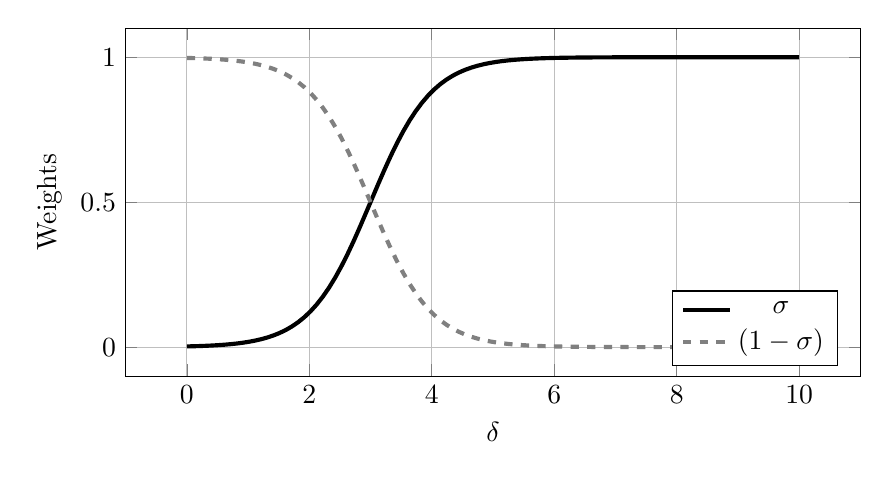
\begin{tikzpicture}%[trim axis left]
		\begin{axis}[
		  width = 0.9\textwidth,
		  height = 6cm,
		  domain = 0.001:10,
		  samples = 100,
		  grid = both,
		  xlabel = $\delta$,
		  ylabel = Weights,
		  legend pos = south east] % customize the axis environment with whatever you want (xmax,ymin,...)	  
		\addplot [color=black, solid, line width=1.5pt] {0.5*tanh(x-3)+0.5}; \addlegendentry{$\sigma$};
		\addplot [color=gray, dashed, line width=1.5pt] {1-(0.5*tanh(x-3)+0.5)}; \addlegendentry{$(1-\sigma)$};
		\end{axis}
	\end{tikzpicture}
	\caption{Plot mit Tikz (ohne Umweg über Matlab)}
\end{figure}
\externalizeOn

\externalizeOff
\begin{figure}[t]
\centering
\tikzsetnextfilename{\currfilebase}% <-- TikzExpernalize PDF gets name of tex-file, otherwise all images are re-compiled in case of reordering the images or adding new ones in between the existing order
\begin{tikzpicture}[align=center,auto,decoration={zigzag}]
%\draw [help lines,dotted,gray,step=5mm] (-4,-3) grid (12,3);

\node[inner sep=0,minimum width=4cm,minimum height=2cm,rotate=0](B)at(0,0){};
\node[yshift=1em] at (B.south){\footnotesize ship};
%% Ship:
\draw[rounded corners=10,thick] (B.east) to (B.70) to (B.north west) to (B.south west) to (B.-70) to (B.east);
\draw[very thick] (B.west)--++(35:-1cm);

%% Hilfslinien
\draw[dashed] (B.west)--node[below,yshift=-1em,pos=0.3]{\footnotesize rudder}++(35:-2cm);
\draw[dashed] ($(B.west)-(2cm,0)$) to ($(B.east)+(2cm,0)$);
\draw[arrow] ($(B.west)-(1.5cm,0)$) arc [start angle=180, end angle=215, radius=1.5cm] node[pos=0.5,left]{$\delta$};

\draw[arrow] (B.east)-- node[at end,below]{\footnotesize ship course} ++(-27.5:2cm);

\draw[arrowreverse] ($(B.east)+(1.5cm,0)$) arc [start angle=0, end angle=-27.5, radius=1.5cm] node[pos=0.5,right]{$\varphi$};

\draw[arrow] (6cm,-1.0cm)--node[right,at end]{$\delta$}++(0,2.5cm);
\draw[arrow] (5.5cm,1cm)--node[below,at end]{$\varphi$}++(6cm,0);
\draw[thick] (6cm,1cm)--++(-20:5.5cm);
\draw[thick,BlueColor] (11cm,1cm) arc [start angle=0, end angle=-20, radius=5cm];
\draw[thick,BlueColor,decorate] ($(6cm,1cm)+(-20:5cm)$) -- node[left,yshift=-1em,text=black]{\footnotesize\emph{sliding mode}} ++(-20:-4cm);
\end{tikzpicture}
\caption{Just a primitive Tikz example.}
\end{figure}
\externalizeOn

\externalizeOff
\begin{figure}[htb]
	% Define block styles
	\tikzstyle{decision} = [diamond, draw, %fill=green!20, 
		text width=4.0em, text badly centered, node distance=2cm, inner sep=0pt]
	\tikzstyle{block} = [rectangle, draw, %fill=green!20, 
	text width=5em, text centered, rounded corners, minimum height=2em]
	\tikzstyle{line} = [draw, -latex']
	\tikzstyle{cloud} = [draw, ellipse, %fill=orange!40,
				 node distance=3cm, minimum height=2em]
	
	\begin{center}
		\begin{tikzpicture}[node distance = 1.4cm, auto, every node/.style={font=\sffamily\scriptsize}]
		% Place nodes
		\node [block] (init) {initialize model};
		\node [cloud, left of=init] (expert) {expert};
		\node [cloud, right of=init] (system) {system};
		\node [block, below of=init] (identify) {identify candidate models};
		\node [block, below of=identify] (evaluate) {evaluate candidate models};
		\node [block, left of=evaluate, node distance=3cm] (update) {update model};
		\node [decision, below of=evaluate] (decide) {is best candidate better?};
		\node [block, below of=decide, node distance=1.9cm] (stop) {stop};
		% Draw edges
		\path [line] (init) -- (identify);
		\path [line] (identify) -- (evaluate);
		\path [line] (evaluate) -- (decide);
		\path [line] (decide) -| node [near start] {yes} (update);
		\path [line] (update) |- (identify);
		\path [line] (decide) -- node {no}(stop);
		\path [line,dashed] (expert) -- (init);
		\path [line,dashed] (system) -- (init);
		\path [line,dashed] (system) |- (evaluate);
		\end{tikzpicture}
	\end{center}
	\caption{Ablaufdiagramm mit Tikz}
\end{figure}
\externalizeOn
%
%
%

